{$\vx = \bmx{c}2\\0\emx$, $\vy = \bmx{c} 1\\3\emx$}
{$\vx+\vy = \bmx{c}3\\3\emx$, $\vx-\vy = \bmx{c} 1\\-3\emx$

Sketches will vary depending on choice of origin of each vector.

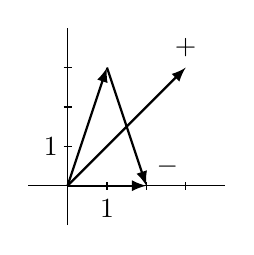
\begin{tikzpicture}[>=latex,scale=.5]
% Draw grid
\draw (-1,0)--(4,0);
\draw (0,-1)--(0,4);
\foreach \x in {1,...,3}
 {\draw (\x,-.1)--(\x,.1);
 }
\foreach \x in {1,...,3}
 {\draw (-.1,\x)--(.1,\x);
 };
\node[below] at (1,-0.1) {1};
\node[left] at (0,1) {1};
%Draw arrows
\draw [->,thick] (0,0)--(2,0) node [below] {\vx};
\draw [->,thick] (0,0) -- (1,3) node [above left] {\vy};
\draw [->,thick] (0,0) -- (3,3) node [above] {$\vx+\vy$};
\draw [->,thick] (1,3) -- (2,0) node [above right] {$\vx-\vy$};
\end{tikzpicture}
}